% arara: lualatex
% arara: sumatrapdf
\documentclass{standalone}
% \usepackage[no-math]{fontspec}
% \setmainfont[Ligatures=TeX]{Times New Roman}
\usepackage{unicode-math}
\unimathsetup{math-style=TeX}
% \setmathfont[range=\mathup/{num}]{Times New Roman}
% \setmathfont[range=\mathit/{greek,Greek}]{Cambria Math}
% \setmathfont[range=\mathup/{greek,Greek}]{Cambria Math}
% \setmathfont[range=\mathit/{latin,Latin}]{Times New Roman}
% \setmathfont[range=\mathup/{latin,Latin}]{Times New Roman}
% \setmathfont[range={"2212,"002B,"003D,"0028,"0029,"005B,"005D,"221A,
% "2211,"2248,"222B,"007C,"2026,"2202,"00D7,"0302,"2261,"0025,"22C5,
% "00B1,"2194}]
% {Cambria Math}
\setmainfont{TeX Gyre Termes}
\setmathfont{TeX Gyre Termes Math}
\usepackage{chemfig}
\begin{document}
\setdoublesep{0.35700 em}  % 'Bond Spacing'
\setatomsep{1.78500 em}    % 'Fixed Length'
\setbondoffset{0.18265 em} % 'Margin Width'
\newcommand{\bondwidth}{0.06642 em} % 'Line Width'
\setbondstyle{line width = \bondwidth, cap = round}
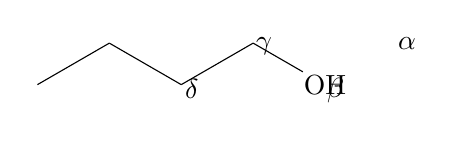
\begin{tikzpicture}[remember picture]
\node at (0,0) {\chemfig{@{d}-[:30]@{g}-[:330]@{b}-[:30]@{a}-[:330]{OH}}};
\draw (a) node[below] {$\alpha$};
\draw (b) node[below] {$\beta$};
\draw (g) node[below] {$\gamma$};
\draw (d) node[below] {$\delta$};
\end{tikzpicture}
\end{document}
